% ****** Start of file apssamp.tex ******
%
%   This file is part of the APS files in the REVTeX 4.1 distribution.
%   Version 4.1r of REVTeX, August 2010
%
%   Copyright (c) 2009, 2010 The American Physical Society.
%
%   See the REVTeX 4 README file for restrictions and more information.
%
% TeX'ing this file requires that you have AMS-LaTeX 2.0 installed
% as well as the rest of the prerequisites for REVTeX 4.1
%
% See the REVTeX 4 README file
% It also requires running BibTeX. The commands are as follows:
%
%  1)  latex apssamp.tex
%  2)  bibtex apssamp
%  3)  latex apssamp.tex
%  4)  latex apssamp.tex
%
\documentclass[%
 reprint,
%superscriptaddress,
%groupedaddress,
%unsortedaddress,
%runinaddress,
%frontmatterverbose, 
%preprint,
%showpacs,preprintnumbers,
%nofootinbib,
%nobibnotes,
%bibnotes,
 amsmath,amssymb,
% aps,
pra,
%prb,
%rmp,
%prstab,
%prstper,
%floatfix,
]{revtex4-1}

\usepackage{graphicx}% Include figure files
\usepackage{dcolumn}% Align table columns on decimal point
\usepackage{bm}% bold math
\usepackage{hyperref}% add hypertext capabilities
%\usepackage[mathlines]{lineno}% Enable numbering of text and display math
%\linenumbers\relax % Commence numbering lines


\def\qp{{q^\prime}}
\def\dul#1{\underline{\underline{#1}}}
\def\ul#1{\underline{#1}}
\def\frvecop#1{\hat{\tilde{\underline{#1}}}}
\def\frmat#1{\tilde{\dul{#1}}}
\def\myeq#1{\stackrel{\mathclap{\tiny\mbox{#1}}}{=}}
\def\frop#1{\hat{\tilde{#1}}}

\def\ket#1{|#1\rangle}
\def\e#1{ e^{#1}}
\def\bra#1{\langle#1|}
\def\av#1{\langle#1\rangle}

\def\tder#1{\frac{d#1}{dt}}
\def\eps{\varepsilon}
\def\nup{\nu^\prime}

\def\aop{\hat{a}}
\def\adop{\hat{a}^\dagger}
\def\dop{\hat{d}}
\def\ddop{\hat{d}^\dagger}
\def\sigop{\hat{\sigma}^-}
\def\sigdop{\hat{\sigma}^+}
\def\Hop{\hat{H}}
\def\Hpop{\hat{H}^\prime}
\def\qp{{q^\prime}}
\def\tp{{t^\prime}}
\def\kappap{{\kappa^\prime}}

\def\thetap{\theta^\prime}

\def\ctil{\tilde{c}}
\def\nn{\nonumber}

\newcommand{\lsz}{\left[}
\newcommand{\rsz}{\right]}
\newcommand{\lk}{\left(}
\newcommand{\rk}{\right)}
\newcommand{\lka}{\left\{}
\newcommand{\rka}{\right\}}
\newcommand{\labs}{\left|}
\newcommand{\rabs}{\right|}
\newcommand{\lla}{\left\langle}
\newcommand{\rra}{\right\rangle}
\usepackage{xcolor}


\def\refeq#1{{\hyperref[#1]{(\ref*{#1})}}}
\def\reffig#1{{\hyperref[#1]{FIG. \ref*{#1}}}}
\def\refsec#1{{\hyperref[#1]{SEC. \ref*{#1}}}}
\def\refno#1{{\hyperref[#1]{\ref*{#1}}}}

\newcommand\note[1]{{\color{red}{#1}}}
%\usepackage[showframe,%Uncomment any one of the following lines to test 
%%scale=0.7, marginratio={1:1, 2:3}, ignoreall,% default settings
%%text={7in,10in},centering,
%%margin=1.5in,
%%total={6.5in,8.75in}, top=1.2in, left=0.9in, includefoot,
%%height=10in,a5paper,hmargin={3cm,0.8in},
%]{geometry}

\begin{document}

\preprint{APS/123-QED}

\title{Difference between a cavity and time-delayed coherent feedback}% Force line breaks with \\
%\thanks{A footnote to the article title}%

\author{Nikolett N\'emet}
\email{nnem614@aucklanduni.ac.nz} %\altaffiliation[Also at ]{Physics Department, XYZ University.}%Lines break automatically or can be forced with \\
\affiliation{The Dodd-Walls Centre for Photonic and Quantum Technologies, New
Zealand}
\affiliation{Department of Physics, 
             University of Auckland, Auckland, New Zealand}
\author{Alexander Carmele}%
 \affiliation{Nichtlineare Optik und Quantenelektronik, Institut f\"ur 
Theoretische Physik, Technische Universit\"at Berlin, Germany}

\author{Scott Parkins}
\affiliation{The Dodd-Walls Centre for Photonic and Quantum Technologies, New
Zealand}
\affiliation{Department of Physics, 
             University of Auckland, Auckland, New Zealand}
             
\author{Andreas Knorr}
\affiliation{Nichtlineare Optik und Quantenelektronik, Institut f\"ur 
Theoretische Physik, Technische Universit\"at Berlin, Germany}

\date{\today}% It is always \today, today,
             %  but any date may be explicitly specified

\begin{abstract}
An article usually includes an abstract, a concise summary of the work
covered at length in the main body of the article. 
\begin{description}
%\item[Usage]
%Secondary publications and information retrieval purposes.
\item[PACS numbers]
May be entered using the \verb+\pacs{#1}+ command.
%\item[Structure]
%You may use the \texttt{description} environment to structure your abstract;
%use the optional argument of the \verb+\item+ command to give the category of each item. 
\end{description}
\end{abstract}

\pacs{Valid PACS appear here}% PACS, the Physics and Astronomy
                             % Classification Scheme.
%\keywords{Suggested keywords}%Use showkeys class option if keyword
                              %display desired
\maketitle

%\tableofcontents

\section{Introduction}
All that we know about feedback...

\begin{itemize}
    \item Fundamental work \cite{Lloyd2000}
    \item General description of coherent vs measurement-based feedback \cite{Jacobs2014}
    \item atom in front of a mirror (sinkL) \cite{Eschner2001,Dorner2002, Beige2002,Tufarelli2014}
    \item Single-delay setup \cite{Wiseman1994}
    \begin{itemize}
        \item squeezing \cite{Gough2009,Iida2012,Kraft2016,Nemet2016}
    \end{itemize}
    \item Multimode setup \cite{Mabuchi2008}
    \item SLH framework \cite{Gough2008}
\end{itemize}

\clearpage
\section{System-environment interaction}
In this paper we focus on systems that are bounded by cavity mirrors and reservoirs-system interactions with some kind of memory intrinsic to them. As we will see the treatment of the two setups in \reffig{fig:setup} stem from the same root, however there is a crucial difference in their treatment which results in distinct behaviours.
\begin{figure}[h!]
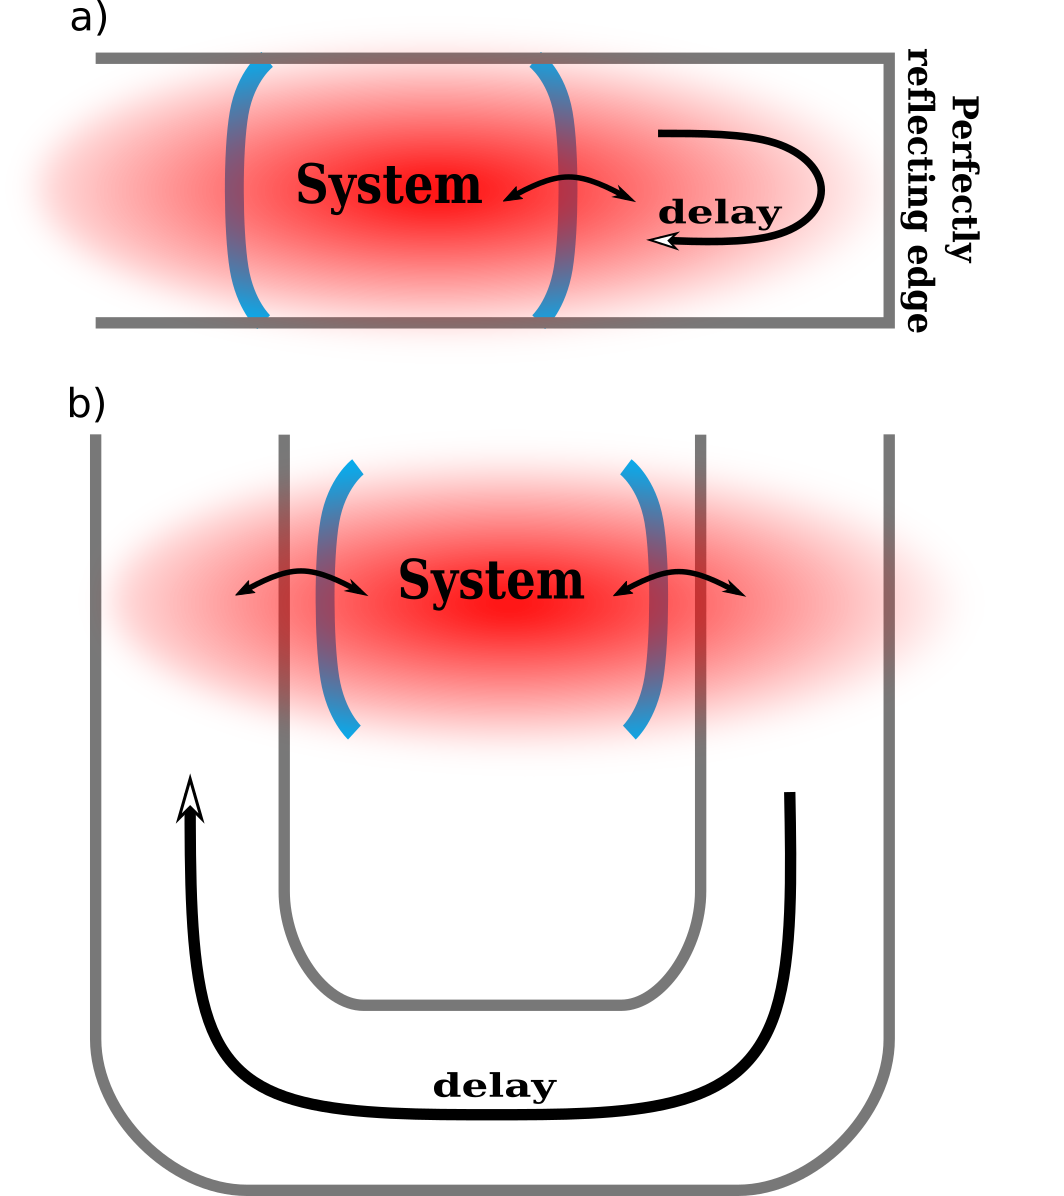
\includegraphics[width=0.4\textwidth]{Setups.png}%
\textit{\textbf{\caption{\linespread{1}\small{Coherent time-delayed feedback types for a System bounded by cavity-mirrors. a) In this multidelay scenario the feedback occurs due to the perfectly reflecting mirror or edge of a waveguide. In this case the bath is confined into a finite space, which results in a discreet set of modes. This can also be interpreted as a coherent feedback signal with delays as multiples of the returning time to the System. b) In the other, single-delay case the feedback occurs due to the coupling of the system to the reservoir at two different spatial points. Here the bath is not confined in any sense, therefore by considering travelling wave modes, the two-point interaction translates into a two-time interaction between the system and the bath. This enforces non-Markovian dynamics with a single delay.
\label{fig:setup}}}}}
\end{figure}

\subsection{Hamiltonian}
In the most general case we consider a System within a cavity with the following Hamiltonian:
\begin{align}
\Hop_1 &= \Hop_S +\Hop_{S-C} + \hbar\omega_c\adop\aop
\end{align}
where $\Hop_S$ describes the system dynamics, $\Hop_{S-C}$ characterizes the interaction between system variables and the cavity, and finally the last term describes the free evolution of the cavity. 

This setup interacts with a discreet or continuous environment through the cavity enforcing a multidelay (MD) or single-delay (SD) dynamics for the System. This interaction can be described as
\begin{align}
\Hop^{(MD)}_{B-S} &= -\sqrt{\frac{\pi}{L}}\sum_{q=0}^\infty\lk\hbar G_q\adop\dop_q + \hbar G^*_q\ddop_q\aop\rk\\
\Hop^{(SD)}_{B-S} &= -\int_{-\infty}^\infty\lk\hbar G(k)\adop\dop_k + \hbar G^*(k)\ddop_k\aop\rk dk
\end{align}
where the factor $\sqrt{\pi/L}$ comes from the difference between discrete and continuous mode operators \cite{Blow1990}. The mode spacing is taken to be $\frac{\pi}{L}$. $\dop_q$ and $\dop_k$ are the discreet and continuous mode operators respectively and $G_q$ and $G(k)$ describe a dispersive coupling between the bath modes and the cavity. \note{exact form of G?}

Now let us consider our system in the interaction frame described by $\Hop_0=\Hop_S+\hbar\omega_c\adop\aop$:%, where the frequency of the cavity mode is tuned to the atomic resonance $\lk \omega_a=\omega_c=\omega_0\rk$:
\begin{align}
\Hop^{\prime(MD)}_{B-S} &= -\sqrt{\frac{\pi}{L}}\sum_{\qp=-q_0}^\infty\lk\hbar G_{\qp}(t)\adop\dop_{\qp} + \hbar G^*_{\qp}(t)\ddop_{\qp}\aop\rk,\\
\Hop^{\prime(SD)}_{B-S} &= -\int_{-\infty}^\infty\lk\hbar G(k,t)\adop\dop_k + \hbar G^*(k,t)\ddop_k\aop\rk dk
\end{align}

In the discreet case, the time-delay associated with a single roundtrip can be defined as:
\begin{align}
\label{eq:tau}
\tau = \frac{2L}{c_0}
\end{align}
whereas in the continuous mode case, the delay is defined as the time that it takes for the light to travel from one point of interaction to the other.

\subsection{Long-delay limit}
In the following we would like to compare these two cases in the long-delay limit. In this case the box, defining the mode spacing of the discreet reservoir is much greater than the cavity including the system. Thus the field leaving the cavity behaves as a wave-packet that travels to the mirror and returns instead of interfering with itself. In \reffig{fig:long_delay} we can see signatures of such behaviour for the single-delay case, when $\tau\approx 5\pi$, however increasing the delay further shows a better qualitative agreement between the single-delay and multidelay case.

\clearpage
\begin{widetext}
\
\begin{figure}[h!]
\centering
\vglue -.2 cm
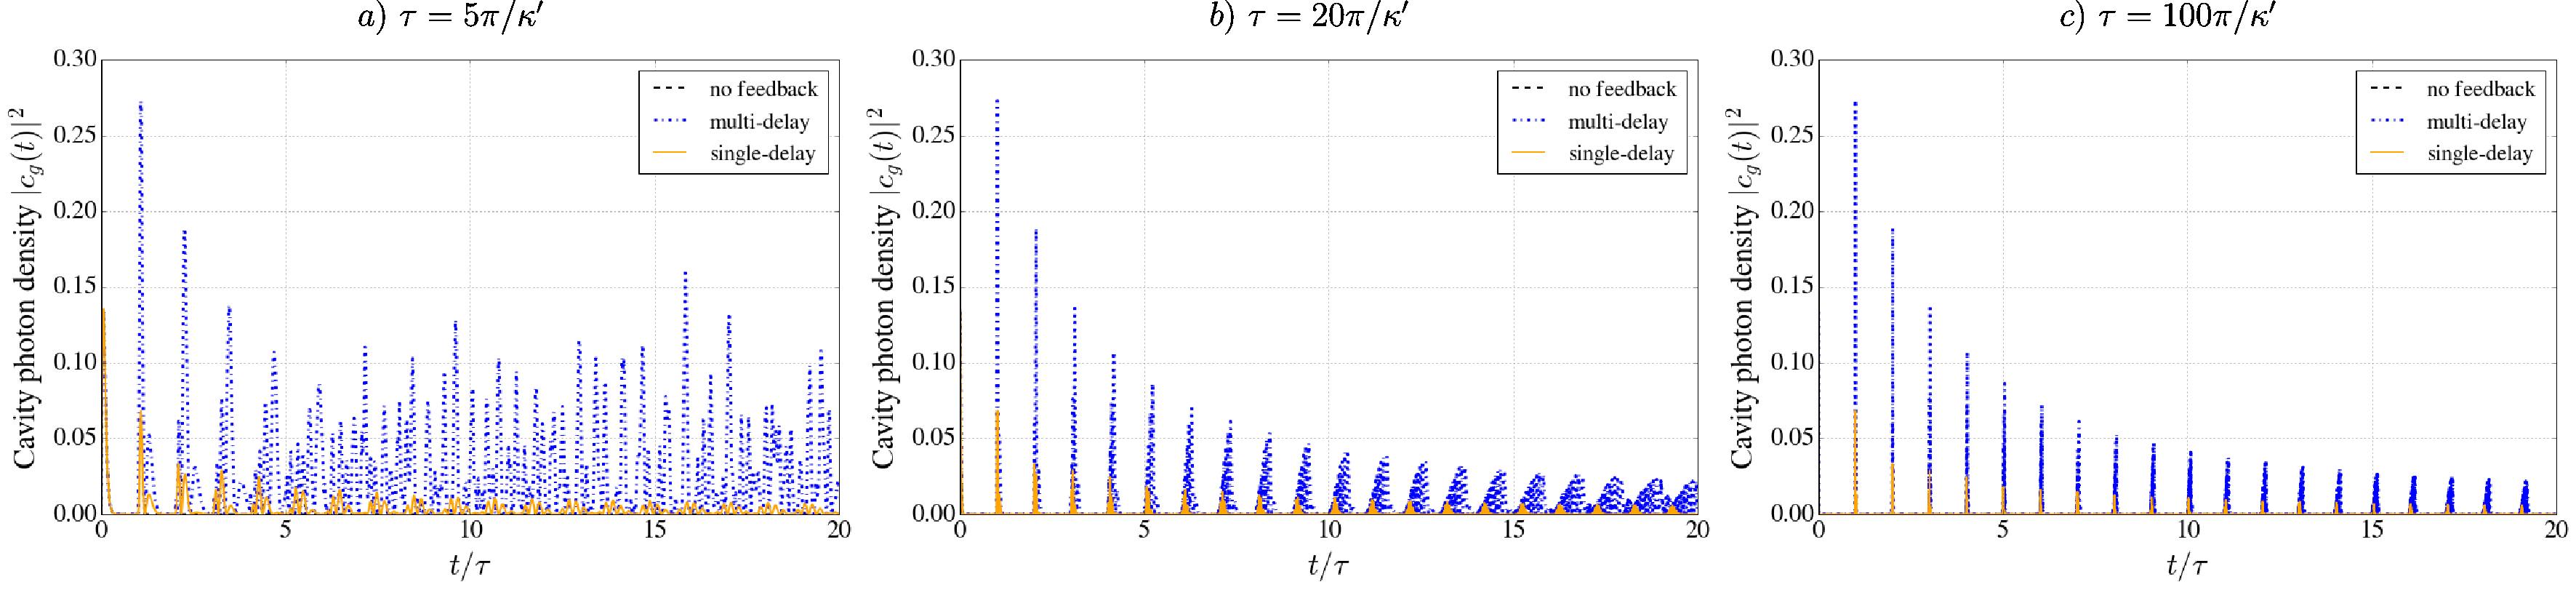
\includegraphics[width=1.0\textwidth]{longdelay_gam=kap=1.png}
\vglue -.2 cm
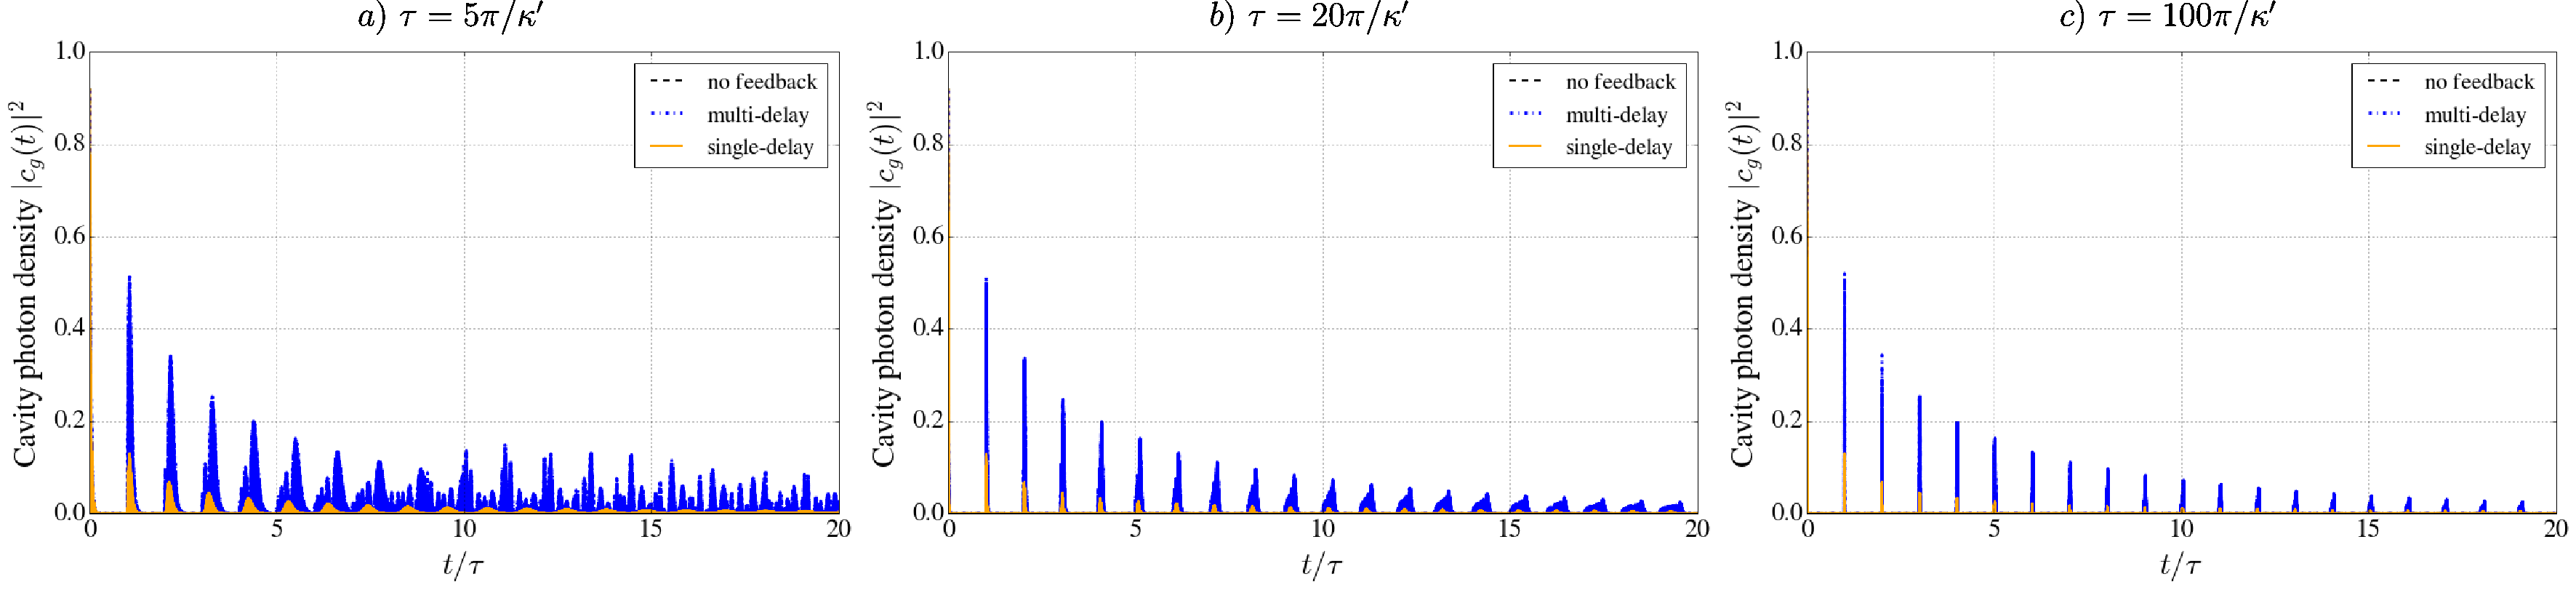
\includegraphics[width=1.0\textwidth]{longdelay_gam=40,kap=1.png}
\vglue -.9 cm
\label{fig:long_delay}
\textit{\textbf{\caption{\linespread{1}\small{Time-evolution of the cavity field for different length of time-delay. In the first row $\gamma=\kappa$, whereas in the second row $\gamma=40\kappa$. The single-delay case is calculated from \cite{Kabuss2015}.}}}}
\vglue -.1 cm
\end{figure}
\end{widetext}

For better comparison, we can zoom in for the individual peaks at multiples of $\tau$ (\reffig{fig:long_delay_zoom}). We can see that although the high-frequency oscillations agree well between the two cases, the multidelay dynamics seems to generate a new pulse with each reflection, whereas the single-delay case preserves the shape of the initial outgoing pulse. \note{Qualitative explanation}

\begin{widetext}
\
\begin{figure}[p]
\centering
\vglue -.2 cm
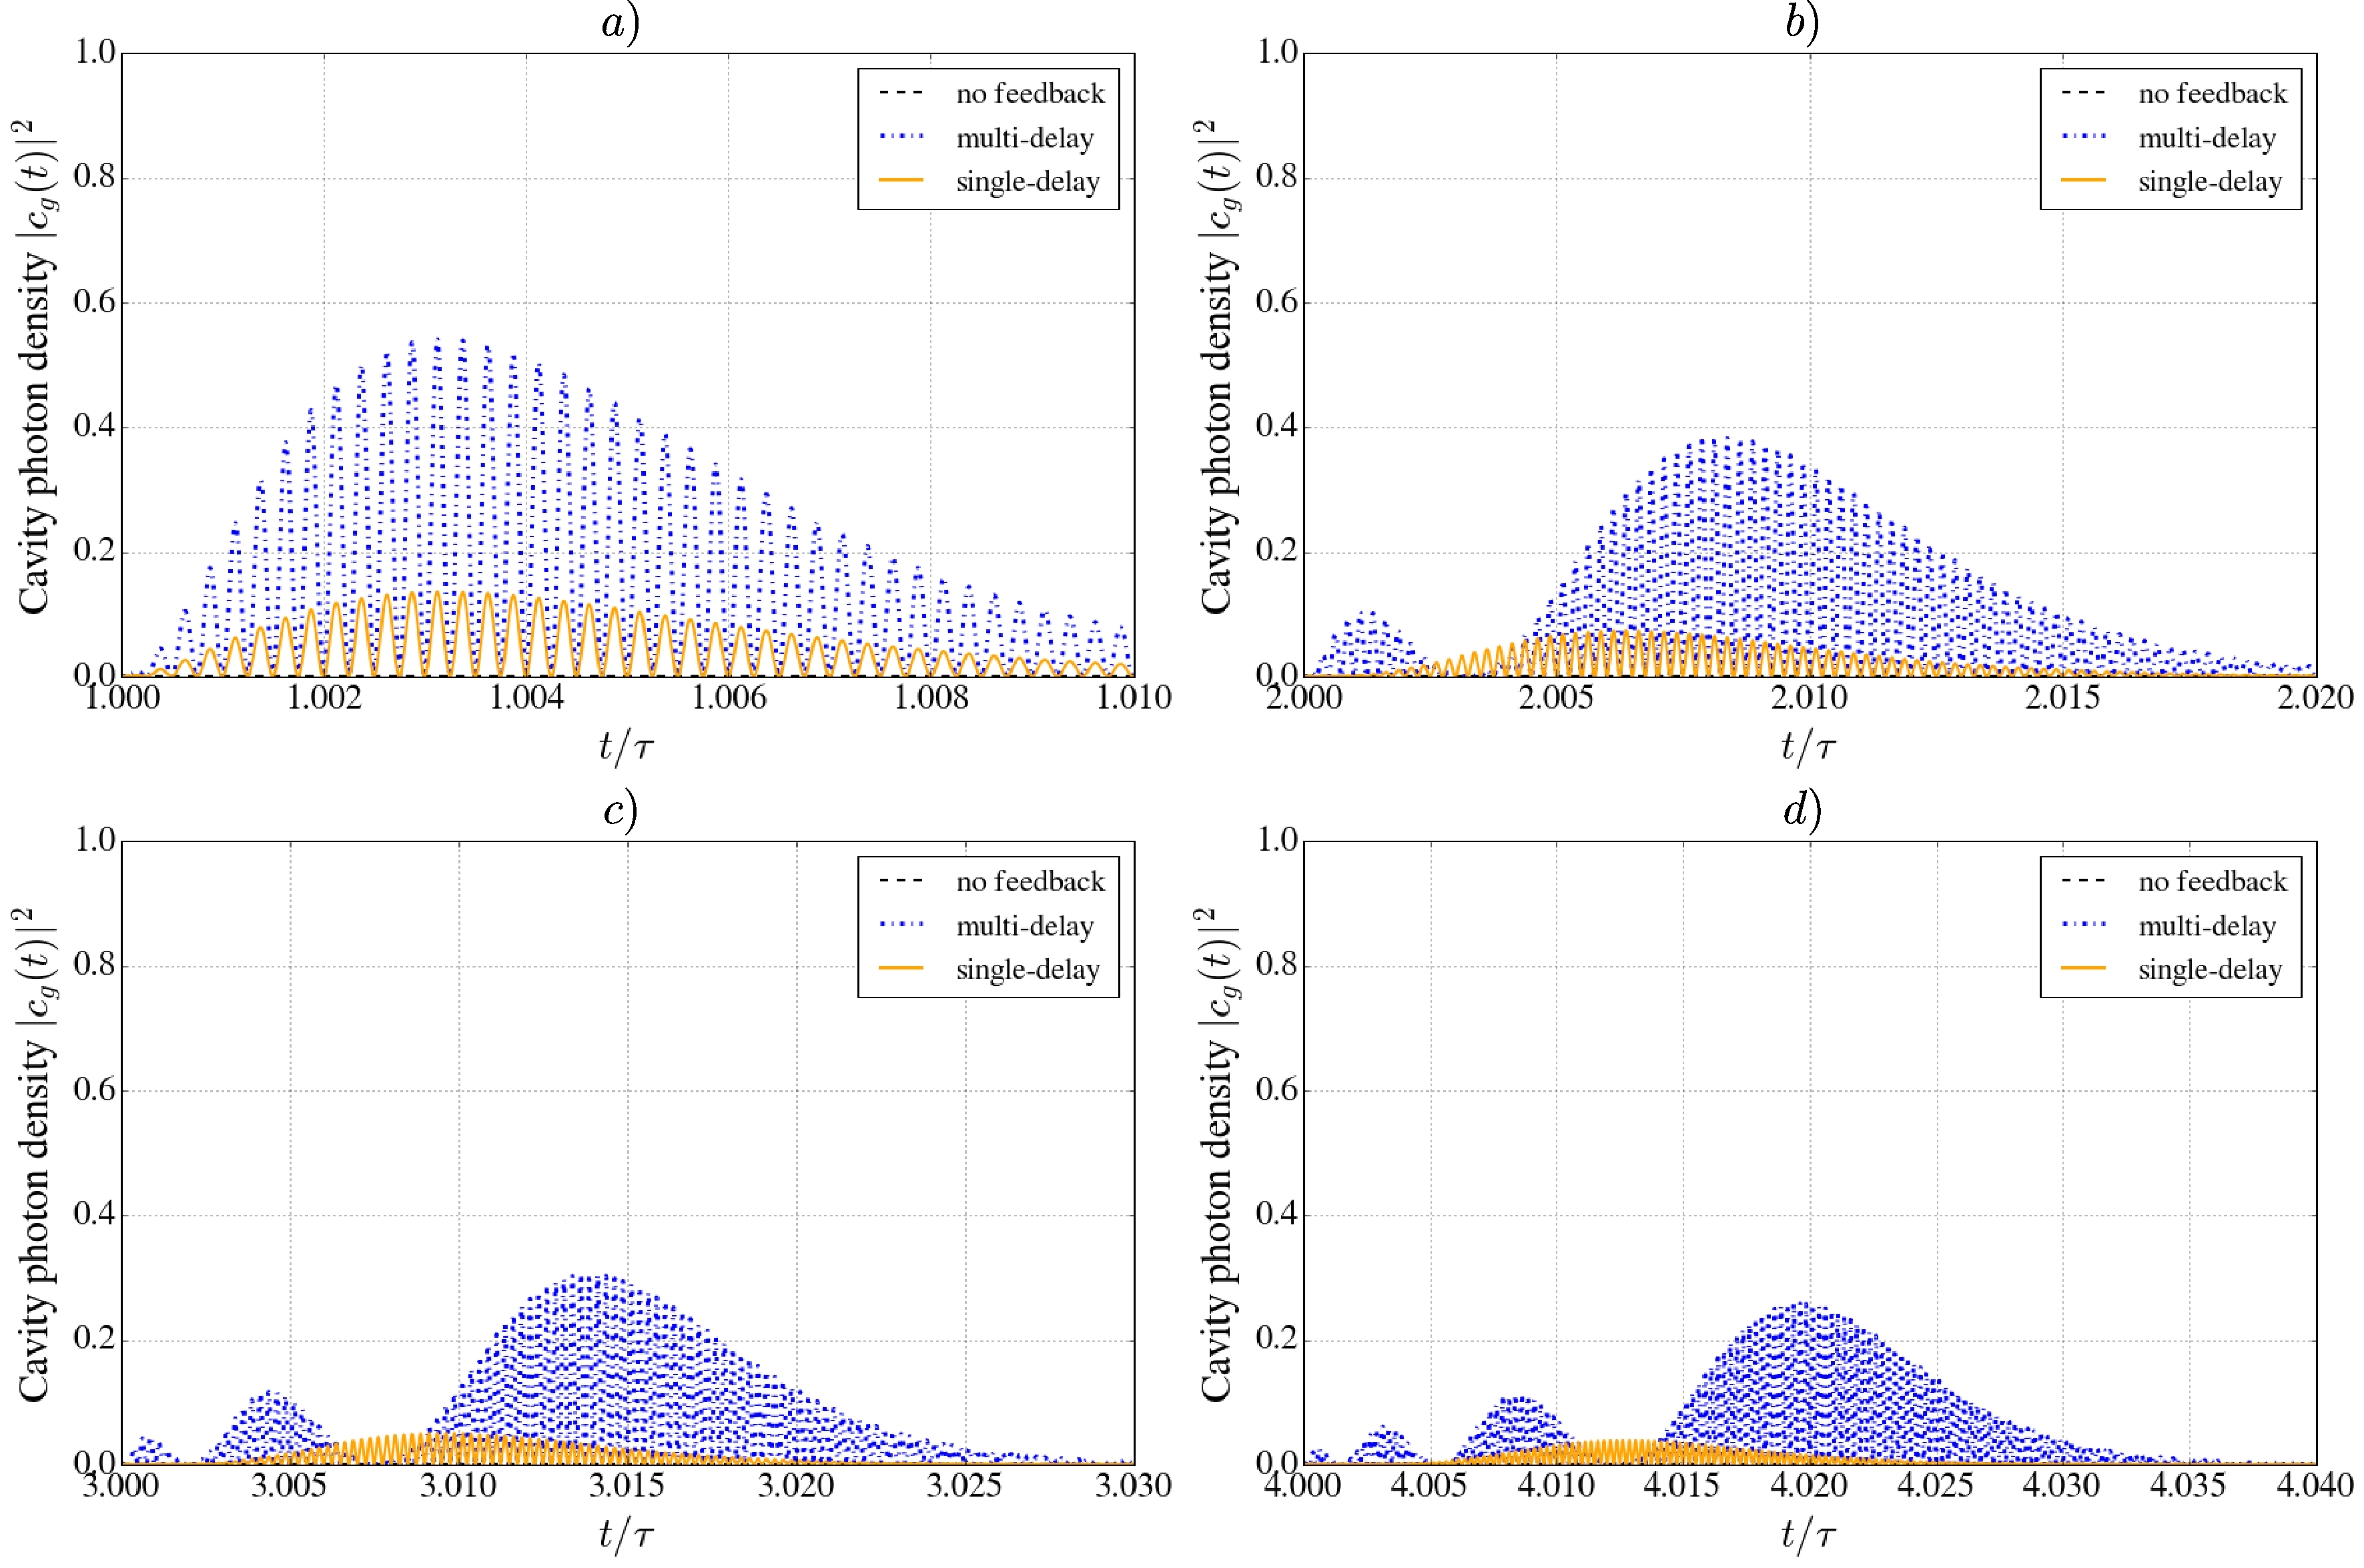
\includegraphics[width=0.8\textwidth]{longdelay_tau=100pi,kap=gam=1.png}
\vglue -.1 cm
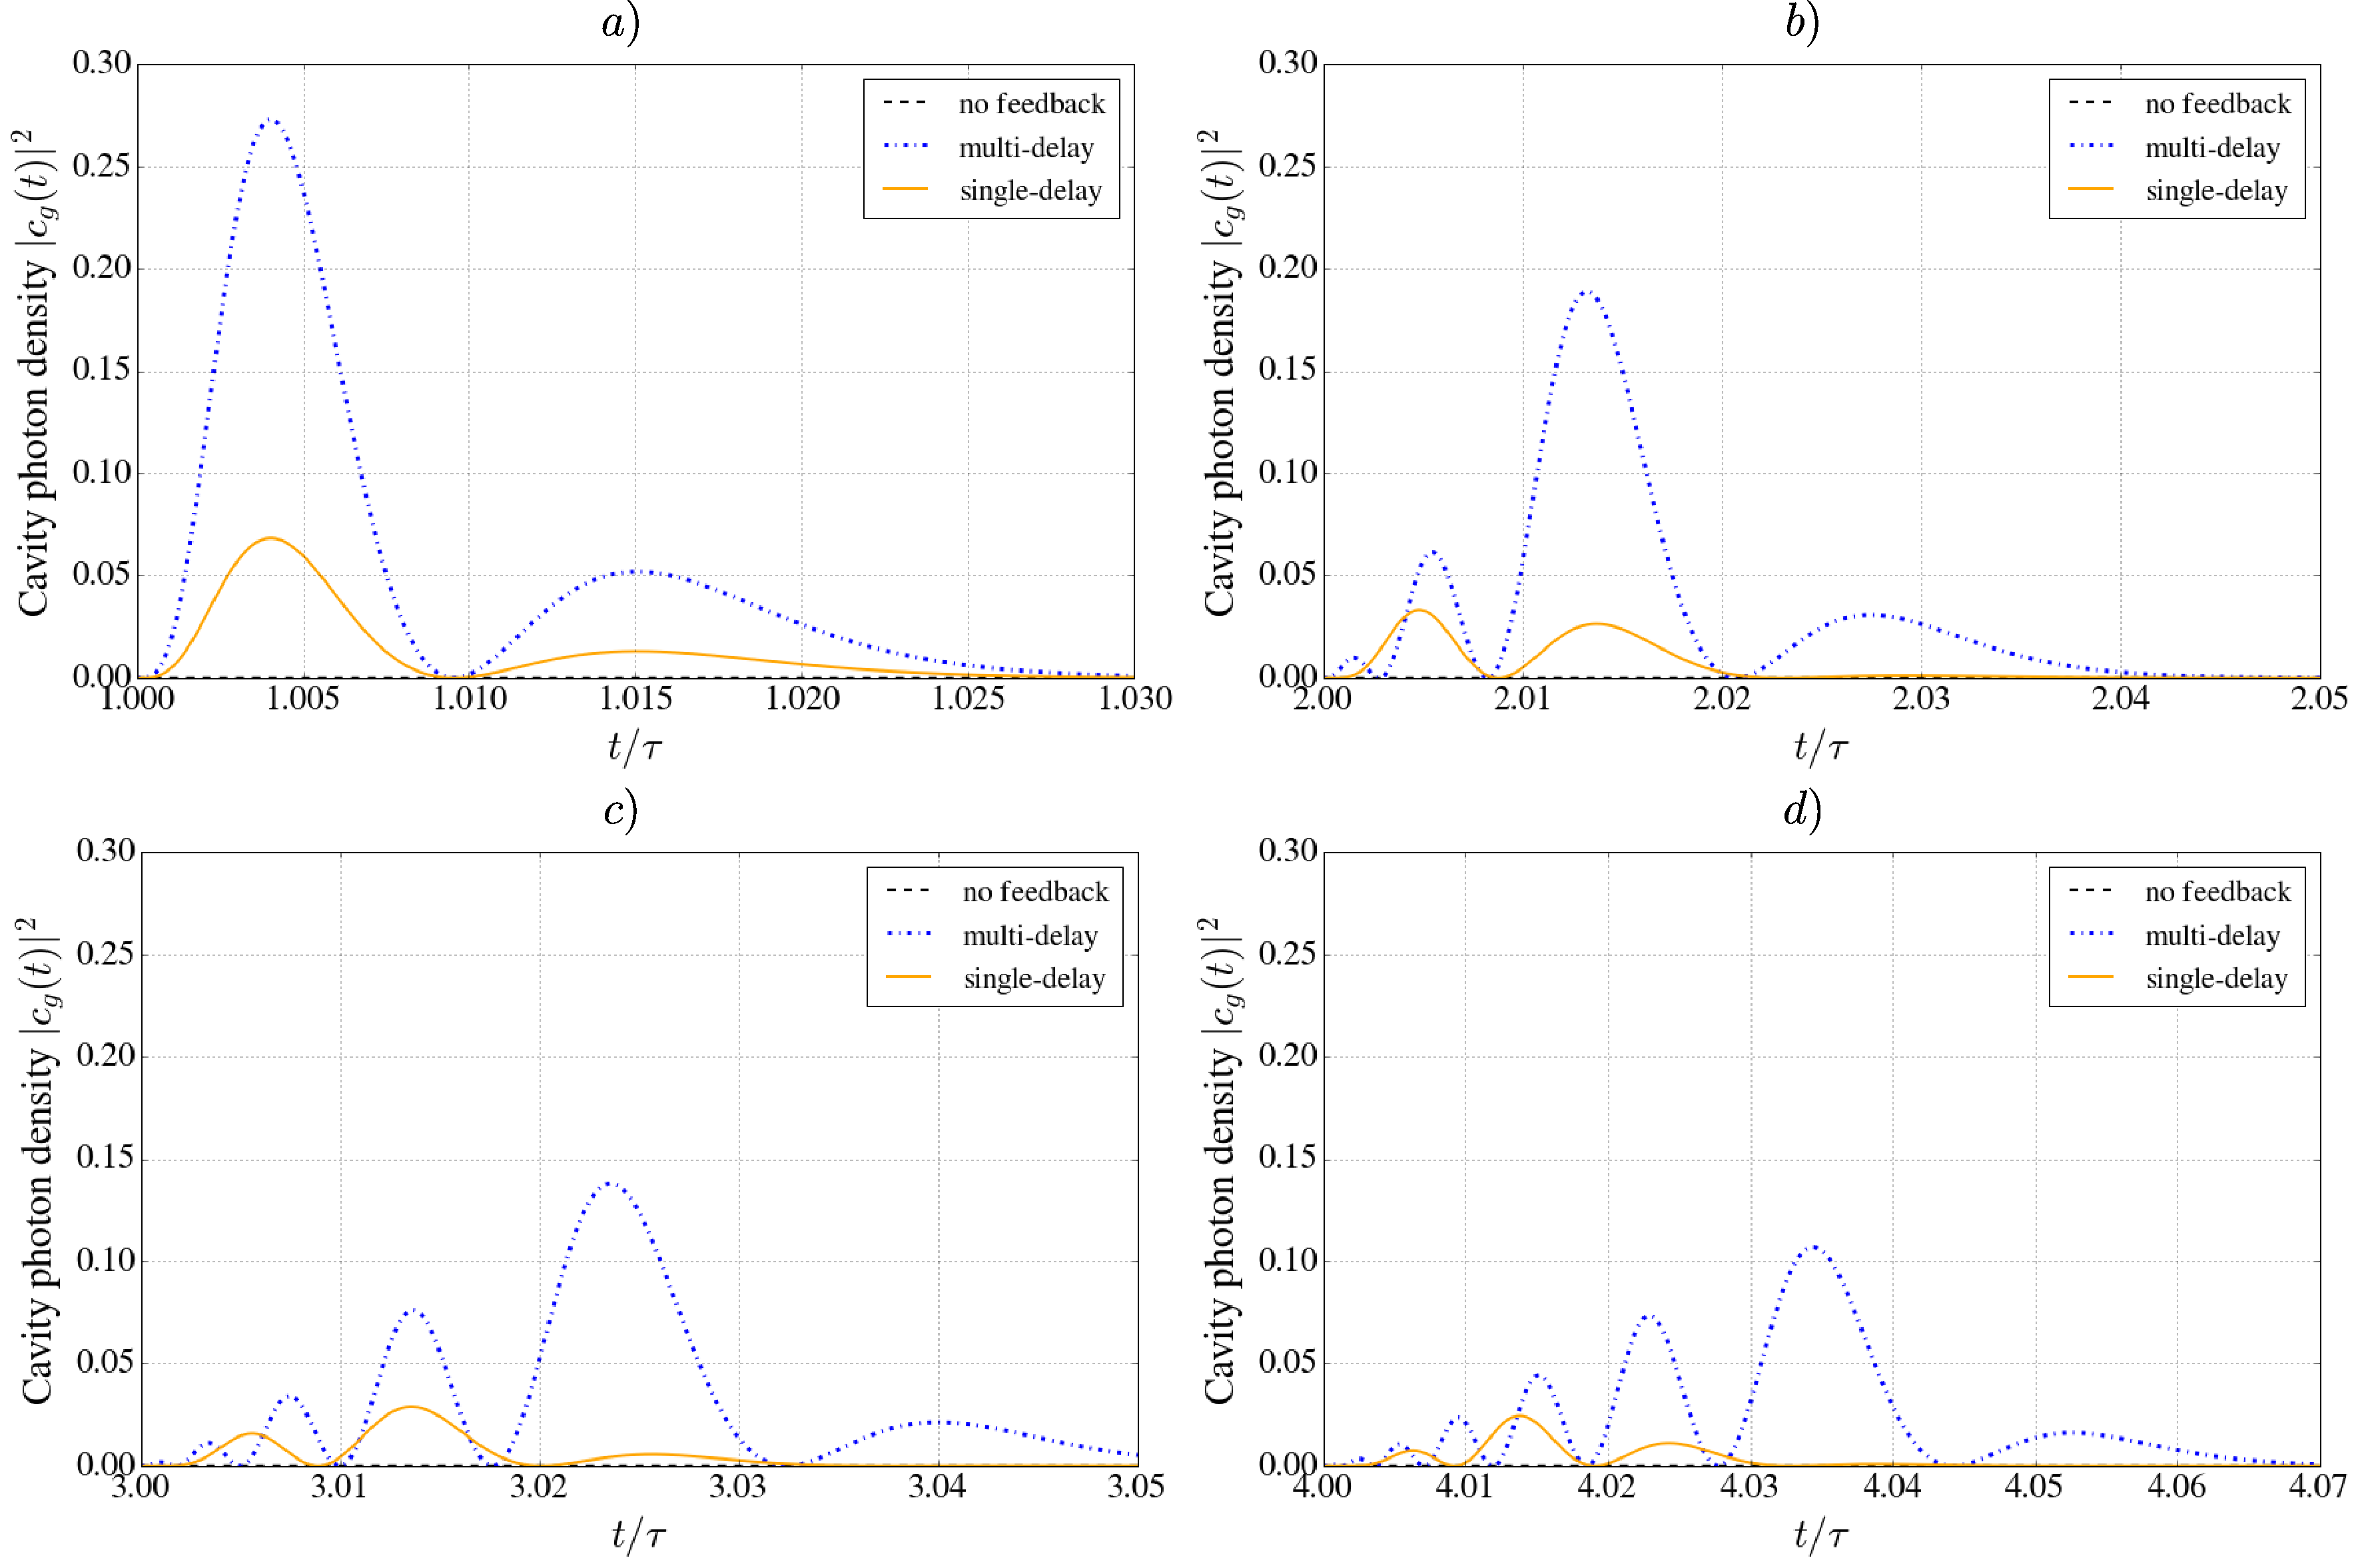
\includegraphics[width=0.8\textwidth]{longdelay_tau=100pi,kap=1,gam=40.png}
\vglue -.9 cm
\label{fig:long_delay_zoom}
\textit{\textbf{\caption{\linespread{1}\small{Different sections of the time-evolution of the cavity field for different length of time-delay. In the upper 4 plots $\gamma=\kappa$, whereas in the lower 4 plots $\gamma=40\kappap$. $\kappa\tau = 100\pi$. The single-delay case is calculated from \cite{Kabuss2015}.}}}}
\vglue -.1 cm
\end{figure}
\end{widetext}

\clearpage
\section{Single excitation limit}
In order to have some analytic insight about the differences between the continuous and discreet case, we assume that there is only a single initially excited atom as a System in the cavity. Thus we assume the Jaynes-Cummings Hamiltonian with the rotating-wave approximation:
\begin{align}
    \Hop_1 = \hbar\omega_a\sigdop\sigop + \hbar\omega_c\adop\aop - \hbar\gamma\lk\sigdop\aop+\adop\sigop\rk
\end{align}
From now on, we show the results for the single-delay case from \cite{Kabuss2015} just for comparison. As there is only a single excitation in the whole setup, the wave-function can be expressed as:
\begin{align}
\ket{\psi(t)^{(MD)}} &= c_e^{(MD)}(t)\ket{e,0,\{0\}} + c_g^{(MD)}(t)\ket{g,1,\{0\}} + \nn\\
&\hspace{.4cm}+\sum_\qp c_{g,\qp}^{(MD)}(t)\ket{g,0,\{\qp\}},\\
\ket{\psi(t)^{(SD)}} &= c_e^{(SD)}(t)\ket{e,0,\{0\}} + c_g^{(SD)}(t)\ket{g,1,\{0\}} + \nn\\
&\hspace{.4cm}+\int c_{g,k}^{(SD)}(t)\ket{g,0,\{k\}}.
\end{align}
Using the Schr\"odinger equation with the Hamiltonians in the interaction picture, we obtain the following time-local equations of motion for the discreet mode case:
\begin{align}
\label{eq:c_e_eq_MD}
\frac{dc_e^{(MD)}}{dt} &= i\gamma c_g^{(MD)}(t),\\
\label{eq:c_g_eq_MD}
\frac{dc_g^{(MD)}}{dt} &= i\gamma c_e^{(MD)}(t) +\nn\\ &\hspace{.4cm}+i\sqrt{\frac{\pi}{L}}\sum_{\qp=-\infty}^{\infty}G_\qp(t)c_{g,\qp}^{(MD)}(t),\\
\label{eq:c_gqp_eq_MD}
\frac{dc_{g,\qp}^{(MD)}}{dt} &= i\sqrt{\frac{\pi}{L}}G^*_\qp(t)c_g^{(MD)}(t).
\end{align}
and for the continuous mode case:
\begin{align}
\label{eq:c_e_eq_SD}
\frac{dc_e^{(SD)}}{dt} &= i\gamma c_g^{(SD)}(t),\\
\label{eq:c_g_eq_SD}
\frac{dc^{(SD)}_g}{dt} &= i\gamma c^{(SD)}_e(t) + i\int G(k,t)c^{(SD)}_{g,k}(t),\\
\label{eq:c_gqp_eq_SD}
\frac{dc^{(SD)}_{g,k}}{dt} &= iG^*(k,t)c^{(SD)}_g(t).
\end{align}


Substituting back the formal integral of \refeq{eq:c_gqp_eq_MD} gives for \refeq{eq:c_g_eq_MD}:
\begin{align}
%\sin^2{\lsz(k_\qp+k_0)L\rsz}\cdot\nn\\
\frac{dc_g}{dt} &= i\gamma c_e(t) - \nn\\
&\hspace{.4cm}-\frac{|G_0|^2\pi}{L}\sum_{\qp=-\infty}^{\infty}
\int_0^te^{-i(\omega_\qp+\Delta_0) (t-\tp)} c_{g}(\tp)d\tp\nn.
\end{align}
where $\omega_\qp = c_0\frac{\qp\pi}{L}=\frac{2\qp\pi}{\tau}$. After exchanging the summation with the integral, we have the following expression for the sum for $\qp$:
%\begin{align}
%&\sin^2{\lsz(k_\qp+k_0)L\rsz} = \sin^2{\lsz\lk\omega_\qp+\omega_0\rk\frac{\tau}{2}\rsz} =\nn\\
%&\hspace{.2cm}= -\frac{1}{4}\lsz e^{i2\qp\pi}e^{i\lk\omega_0+\Delta\rk\tau}+e^{-i2\qp\pi}e^{-i\lk\omega_0+\Delta\rk\tau}-2 \rsz=\nn\\
%&\hspace{.2cm}=\frac{1-\cos{\lsz\lk\omega_0+\Delta\rk\tau\rsz}}{2}=\sin^2{\lsz\frac{\omega_0+\Delta}{2}\tau\rsz}.
%\end{align}
%Thus this part is not dependent on frequency, therefore we can evaluate the rest separately
\begin{align}
&\sum_{\qp=-\infty}^{\infty}e^{-i(\omega_\qp+\Delta_0) (t-\tp)} =\nn\\
&\hspace{.2cm}= e^{-i\Delta_0 (t-\tp)}\sum_{\qp=-\infty}^{\infty}e^{-i\qp 2\pi \frac{t-\tp}{\tau}} = \nn\\
&\hspace{.2cm}=\tau e^{-i\Delta_0 (t-\tp)}\sum_{\qp = -\infty}^\infty\delta\lk t-\tp-\qp\tau\rk,
\end{align}
where we have used the Fourier series identity for the Dirac comb \note{(reference?)}. Therefore the equation for $c_g^{(MD)}$ updates as follows:
\begin{align}
\frac{dc_g^{(MD)}}{dt} &= i\gamma c_e^{(MD)}(t) -\frac{|G_0|^2\pi\tau}{L}\cdot\nn\\%\sin^2{\lsz\frac{\omega_0+\Delta}{2}\tau\rsz}\cdot\nn\\
&\hspace{0.0cm}\cdot
\sum_{\qp=-\infty}^{\infty}\int_0^t\delta\lk t-\tp-\qp\tau\rk e^{-i\Delta_0(t-\tp)} c_{g}^{(MD)}(\tp)d\tp.\nn
\end{align}
The range of integration excludes the non-causal values of $\qp<0$. The special behaviour of Dirac-delta on the limits, gives a factor of $1/2$ for $\qp=0$, thus:
\begin{align}
\frac{dc_g^{(MD)}}{dt} &= i\gamma c_e^{(MD)}(t) - \underbrace{\frac{2|G_0|^2\pi}{c_0}}_{4\kappa}\cdot\\%\sin^2{\lsz\frac{\omega_0+\Delta}{2}\tau\rsz}\cdot\\
&\hspace{-1cm}\cdot\lka\sum_{\qp=0}^{\infty}e^{-i\Delta_0\qp\tau} c_{g}^{(MD)}(t-\qp\tau)\Theta(t-\qp\tau)-\frac{1}{2}c_g^{(MD)}(t)\rka,\nn
\end{align}
which means that each roundtrip contributes with its corresponding delay to the time-evolution. This is quite different from the single-delay case, where the system only interacts with one of its past versions via the environment:
\begin{align}
\frac{dc_g^{(SD)}}{dt} &= i\gamma c_e^{(SD)}(t) - 2\kappa\lsz c_g^{(SD)}(t)-\right.\\ &\left.\hspace{3cm}-e^{i\Delta_0\tau}c_{g}^{(SD)}(t-\tau)\Theta(t-\tau)\rsz,\nn
\end{align}

In both cases $\Delta_0\tau$ defines the phase relationship of the output and input fields at different times. In the single-delay case $\phi=\Delta_0\tau=0$ the interference between the present and past field of the cavity can enhance the decay of the cavity field. $\phi=\pi$ on the other hand relates to a suppressed decay.

\clearpage
\subsection{Special points in the stability landscape}
In a previous paper stabilization of Rabi oscillations was found for the single-delay case \cite{Kabuss2015}. This can be identified as a pole on the stability landscape with no real part. In order to investigate whether we can find such special parameter sets for the multidelay case, we look at the Laplace Transform of the equations of motion derived in the previous section.
\begin{align}
\label{eq:lap_ce}
s\ctil_e^{(MD)}(s) &= 1+i\gamma\ctil_g^{(MD)}(s)\\
\label{eq:lap_cg}
s\ctil_g^{(MD)}(s) &= i\gamma\ctil_e(s) -\nn\\
&\hspace{.3cm}-4\kappa\ctil_g^{(MD)}(s)\lsz\sum_\qp e^{-\qp(s+i\Delta_0)\tau}-\frac{1}{2}\rsz
\end{align}

\paragraph{$t<\tau$}
Before the emitted light field can reach the cavity, the system evolves as if there was no reflecting edge.
\begin{align}
\ctil_g^{(0)}(s) = \frac{i\gamma}{s^2+\gamma^2+2\kappa s}
\end{align}
with poles at 
\begin{align}
-\kappa\pm i\gamma\sqrt{1-\frac{\kappa^2}{\gamma^2}}
\end{align}
that gives a time-dependent solution
\begin{align}
c_g^{(0)}(t) = i\gamma\frac{\sin{\lsz\sqrt{1-\frac{\kappa^2}{\gamma^2}}\gamma t\rsz}}{\sqrt{1-\frac{\kappa^2}{\gamma^2}}}e^{-\kappap t},
\end{align}
which means damped oscillations with a shifted frequency both depending on the coupling strength between the cavity and the external modes. The same happens for the single-delay case.

\paragraph{$\tau<t\leq 2\tau$}
In the next time period, after $\tau$, the time-evolution resembles the single-delay case:
\begin{align}
\ctil_g^{(1)(MD)}(s) = \frac{i\gamma}{s^2+\gamma^2+2\kappa s\lk1+2e^{-(s+i\Delta_0)\tau}\rk}
\end{align}
which looks like as if we haveinfinite poles. However, there is some difference in the ratio between the recurring field and the original decay. For the single-delay case we have
\begin{align}
\ctil_g^{(1)(SD)}(s) = \frac{i\gamma}{s^2+\gamma^2+2\kappa s\lk1-e^{-(s+i\Delta_0)\tau}\rk}
\end{align}
once we passed $\tau$. This feedback control supports recovered Rabi oscillations for $(\Delta_0+\gamma)\tau=2n\pi,\  (n\in \mathbb{N})$.

\paragraph{Long-time limit}
In general the solution at $n\tau\le t<(n+1)\tau$ has the following form:
\begin{align}
\ctil_g^{(n)}(s) = \frac{i\gamma}{s^2+\gamma^2-2\kappa s+4\kappa s\sum_{\qp=0}^{n}e^{-\qp(s+i\Delta_0)\tau}}.
\end{align}
Here setting the denominator to zero provides the poles of the stability landscape, which determine the dynamics. Recovered Rabi oscillations or persistant oscillations in general would mean that we have a pole at $s_{osc}=\pm i\mu$. Substituting $s_{osc}$ back and setting the denominator to 0 provides the following:
\vspace{-.4cm}
\begin{align}
-\mu^2+\gamma^2\mp i2\kappa \mu\lk 1-2\sum_{\qp=0}^{n}e^{\mp i\qp(\mu+\Delta_0)\tau}\rk&=0\\
\sum_{\qp=0}^n \cos{\lsz\mp \qp(\mu+\Delta_0)\tau\rsz} &= \frac{1}{2}.\\
-\mu^2+\gamma^2-4\kappa\mu\sum_{\qp=0}^n \sin{\lsz\mp \qp(\mu+\Delta_0)\tau\rsz}&=0
\end{align}
In case of $\mu=\gamma$, which was reported in \cite{Kabuss2015}, in the long time limit, the sum turns into an infinite geometric series. However the absolute value of the individual terms are 1, which means that the sum does not converge. Thus no time-delay can satisfy this requirement. Similarly, in the general case, the condition is given for a non-convergent cosine series.

\subsection{Weak coupling regime}

After finding an appropriate value of the time-delay, coherent cavity-assisted excitation exchange can be observed between the two-level system and the external modes
\begin{widetext}
\ 
\begin{figure}[h!]
\centering
\vglue -1.3 cm
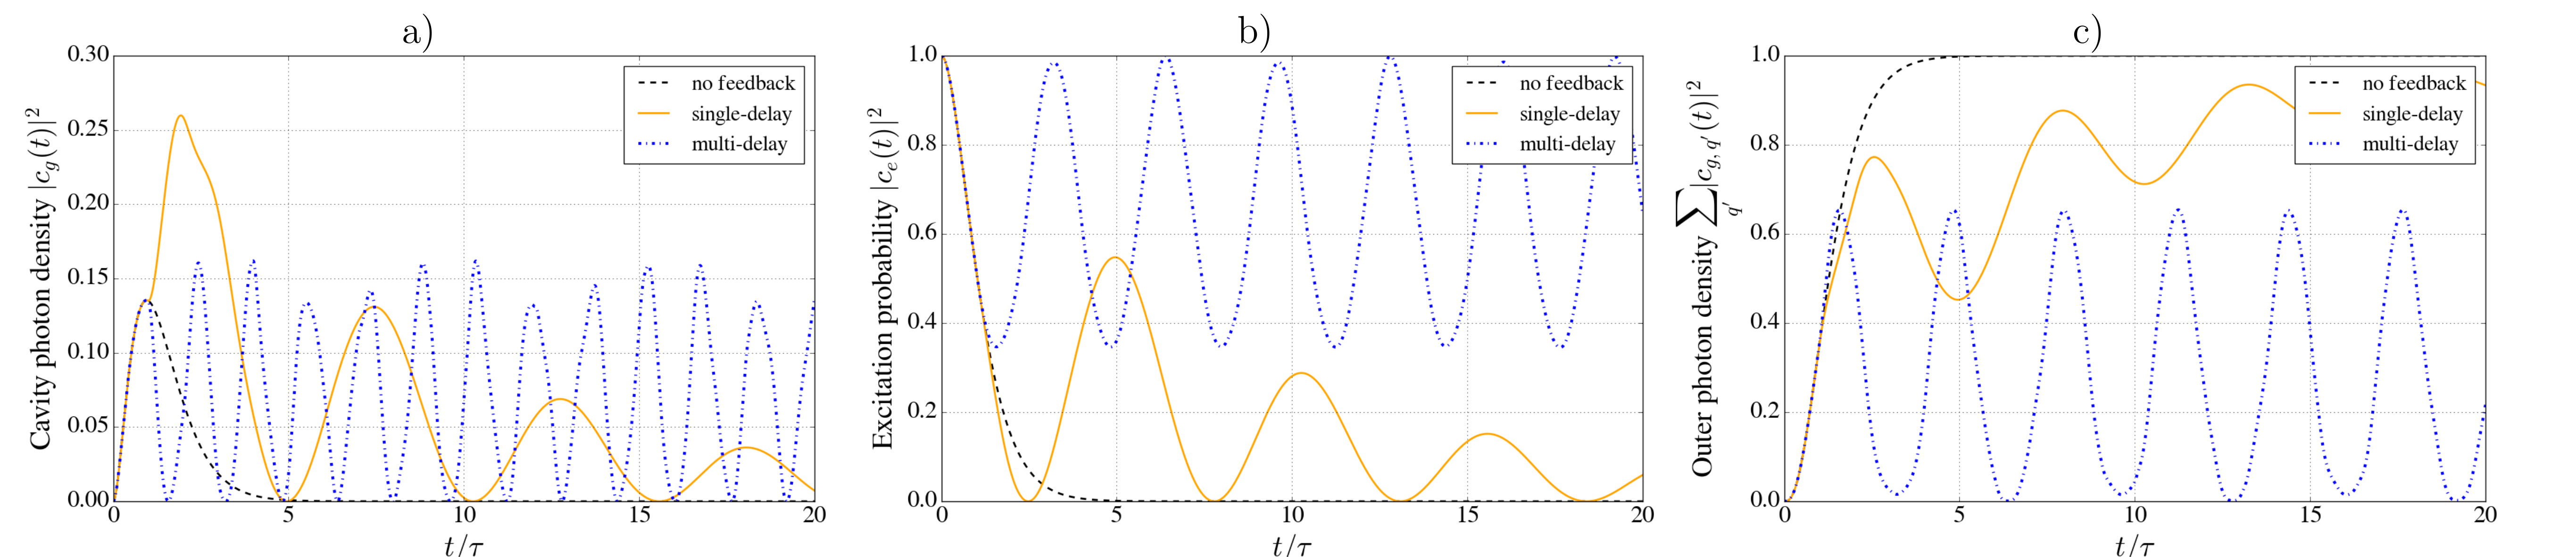
\includegraphics[width=1.0\textwidth]{longtime_kap=2,gam=1,tau=pip3.png}
\vglue -1 cm
\label{fig:weak_envtls}
\textit{\textbf{\caption{\linespread{1}\small{Time-evolution of different excitation probabilities, when $\gamma=\kappap, \tau=\pi/3\gamma$ in the long-time limit. The single-delay case is calculated from \cite{Kabuss2015}.}}}}
\vglue -.4 cm
\end{figure}
\end{widetext}

\note{The frequency of oscillations depend linearly on $\gamma$ and inversely on $\kappa$. Why?}

\clearpage
\subsection{Strong coupling regime}
Collapse and revival
\note{Check the spacing of the revivals! How can we understand them in general?}
\begin{widetext}
\ 
\begin{figure}[h!]
\centering
\vglue -1.2 cm
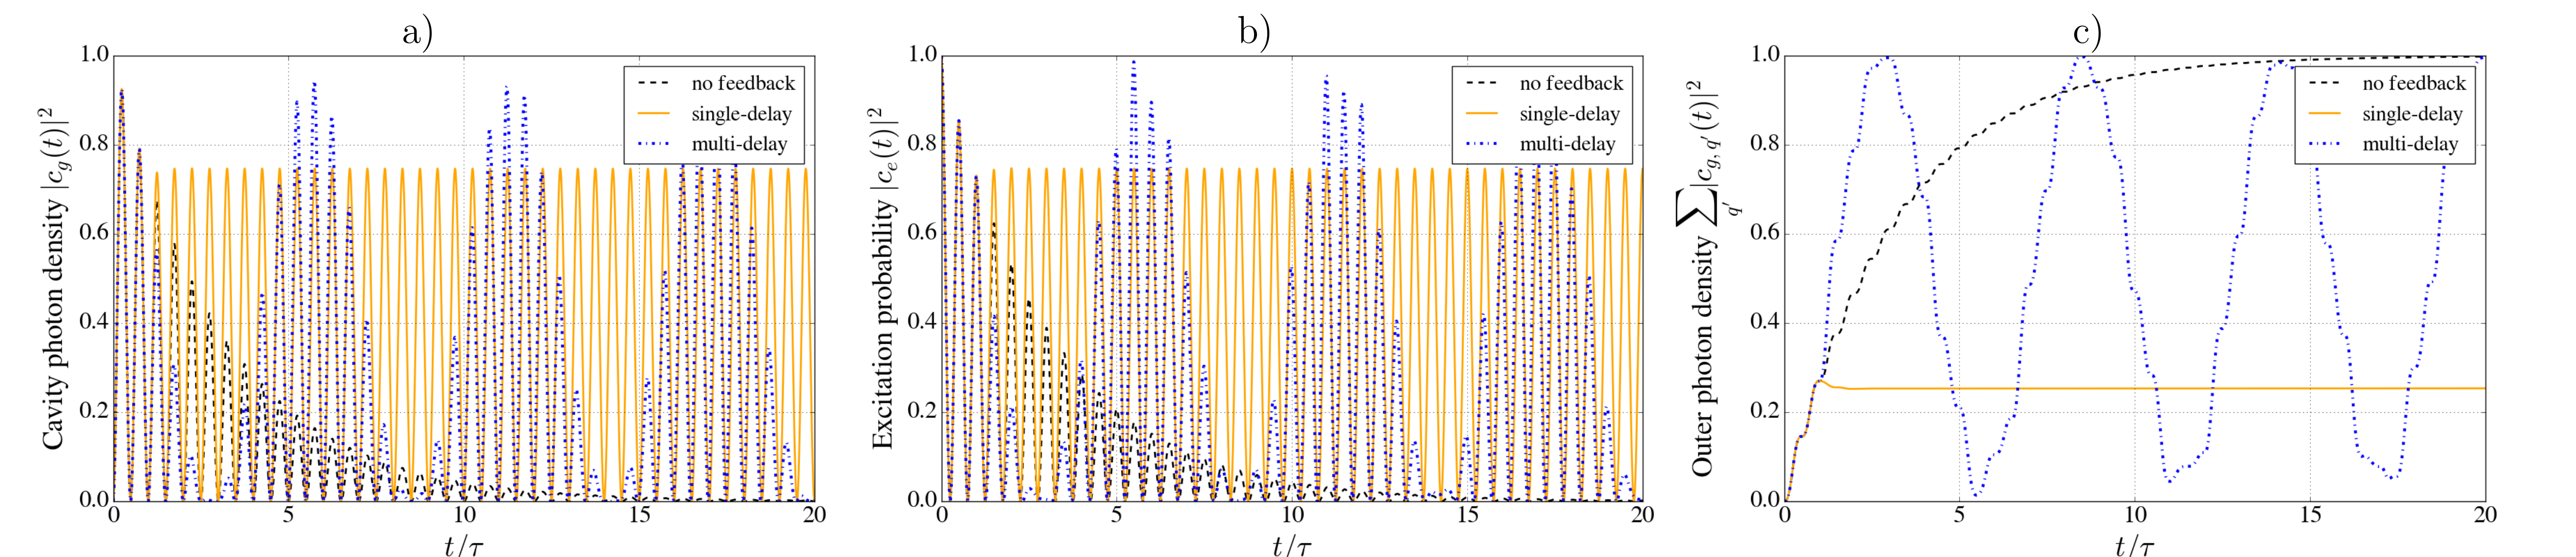
\includegraphics[width=1.0\textwidth]{longtime_kap=2,gam=40,tau=2pip40}
\vglue -1 cm
\label{fig:longgam40_prev}
\textit{\textbf{\caption{\linespread{1}\small{Time-evolution of different excitation probabilities, when $\gamma=40\kappap$ in the long-time limit. The single-delay case is calculated from \cite{Kabuss2015}.}}}}
\vglue -.3 cm
\end{figure}
\end{widetext}

\section{Dark states and excitation trapping}
\subsection{Excitation trapping in the multidelay case}
\begin{figure}[h!]
\centering
\vglue -.2 cm
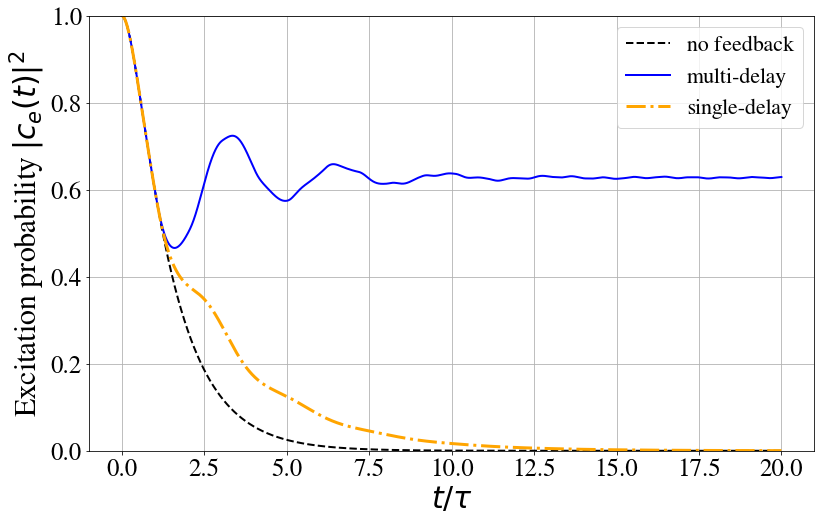
\includegraphics[width=0.45\textwidth]{trapped.png}
\vglue -.8 cm
\label{fig:strong_cavtls}
\textit{\textbf{\caption{\linespread{1}\small{Time-evolution of the cavity field for different length of time-delay, when $\gamma=\kappa=2\pi MHz$. The single-delay case is calculated from \cite{Kabuss2015}.}}}}
\vglue -.1 cm
\end{figure}
\note{Can I show the trapping with the Laplace transform solution $c_e^{(MD)}$?}

\subsection{Single mode theory: Normal modes}
\begin{figure}[h!]
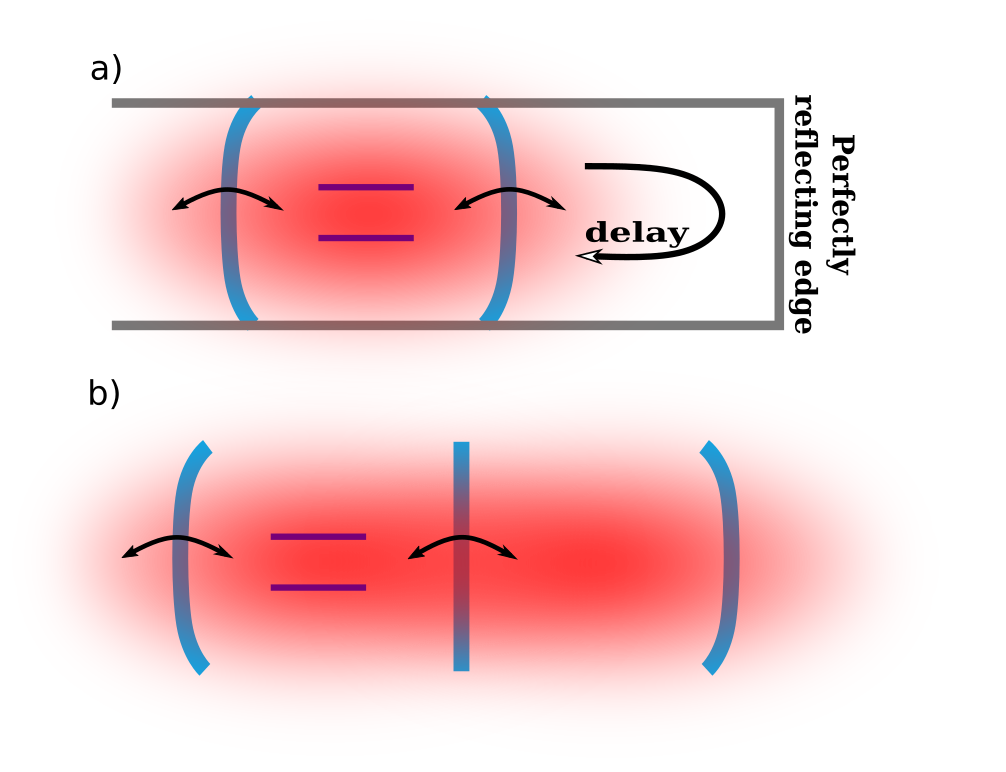
\includegraphics[width=0.45\textwidth]{Coupled_cav.png}%
\vglue -.9 cm
\textit{\textbf{\caption{\linespread{1}\small{{a) Multidelay feedback setup with an atom inside the cavity. b) Coupled cavity-qed with a single atom in one of the cavities.}}}}
\label{fig:CC}}
\end{figure}

The multidelay cavity can also be considered as a multimode cavity coupled to a cavity-QED system (\reffig{fig:CC} b)). In case of two cavities coupled to each other with a mode frequency matching the atomic resonance in the first cavity, we can look at the equations of motion in the weak driving limit. The following normal modes can be observed in the frame rotating by the atomic resonance frequency:
\begin{align}
    \ket{B_\pm} &= \frac{1}{\sqrt{2}\xi}\lk \gamma\ket{A} \pm \xi\ket{C_1}+G_0\ket{C_2}\rk\\
    E_{B_\pm} &= \pm\hbar\xi\\
    \ket{D} &= \frac{1}{\xi}\lk -G_0\ket{A} +\gamma\ket{C_2}\rk\\
    E_D &= 0 \\   
    \xi&=\sqrt{\gamma^2+G_0^2}
\end{align}
where $\ket{B_\pm}$ are bright states and $\ket{D}$ is dark to the leaky cavity. $\ket{C_i}$ represent a coherent excitation of cavity 1 and 2, and $\ket{A}$ represent the state of the atom in cavity 1. $\gamma$ is the coupling strength between cavity 1 and the atom as before, and $G_0=2\sqrt{\frac{\kappa c_0}{\pi}}$ describes the interaction strength between the two cavities.

As the only decay considered here is that of cavity 1, an initially excited atom can preserve some of its excitation due to the existence of the above mentioned dark state. All the other state contributions decay away, and therefore the stronger the cavities are coupled compared to the cavity-atom coupling, the more excitation is preserved in the atom.

Due to the similarity between this coupled-cavity model and our multidelay proposal, a very similar dynamics can be observed. The initially excited atom's state is preserved with the help of the outer confined reservoir.

\subsection{No trapping in single-delay case}
\note{Can I show the lack of trapping with the Laplace transform solution $c_e^{(SD)}$?}

\section{Contribution of the control phase}
The main difference between the two feedback cases is that while in the single-delay case a single well-defined phase determines the interference behaviour at the mirrors, in the multimode case, no such phase can be given. In this latter case, we can only talk about a phase with which a single roundtrip contributes.

In the single-delay case the past field can be coupled back in a completely coherent way due to an entirely imaginary contribution. However, in the multimode case, even if there is a purely imaginary contribution from a single roundtrip, there will be incoherent, lossy contributions involved due to the multiples of this phase.

\note{Can we say more about this? What happens as these multiples of the same phase interfere? Is it always a collapse-revival feature?}

\clearpage
\section{Cavity output spectra}
The Laplace transform of the cavity field derived from the time-local system of equations \refeq{eq:c_e_eq_MD}-\refeq{eq:c_gqp_eq_MD} with the extra damping term:
\begin{align}
\tilde{c}_g^{(TL)}(s) &= i\gamma\lsz s^2+\gamma^2+\kappa_1s+\right.\nn\\
&\hspace{.4cm}\left.+4\kappa s\sum_{\qp=-\frac{N-1}{2}}^{\frac{N-1}{2}}\frac{1}{s\tau+\phi+i2\qp\pi}\rsz^{-1}\nn\\
\tilde{c}_g^{(TL)}(-i\omega) &= i\gamma\lsz -\omega^2+\gamma^2-i\omega\kappa_1+\right.\nn\\
&\hspace{-.4cm}\left.+4\kappa\omega \sum_{\qp=-\frac{N-1}{2}}^{\frac{N-1}{2}}\frac{1}{\omega\tau-\phi-2\qp\pi}\rsz^{-1}
\end{align}
where we consider only $N$ number of modes, which are the closest to the cavity resonance and $\phi=\Delta_0\tau$. 

From the delayed model, described by Laplace transforms \refeq{eq:lap_ce} and \refeq{eq:lap_cg} we obtain in the damped case:
\begin{align}
\ctil_g^{(MD)}(s) &= i\gamma\lsz s^2+\gamma^2+\kappa_1s +\right.\nn\\
&\hspace{.7cm}\left.+ 4\kappa s\lk\sum_{\qp=0}^\infty e^{-\qp(s\tau+\phi)}-\frac{1}{2}\rk\rsz^{-1} \nn\\
\ctil_g^{(MD)}(-i\omega)&=i\gamma\lsz -\omega^2+\gamma^2-i\omega\kappa_1 +\right.\nn\\
&\hspace{1cm}\left.+ \frac{2\kappa\omega}{\tan{\lsz\lk\omega\tau-\phi\rk/2\rsz}}\rsz^{-1}
\end{align}
The sum in this expression is convergent if $s$ has a real part. \note{So does it converge or not?} 
The spontaneous emission spectra can be expressed as:
\begin{align}
S(\omega) = \frac{\kappa_1}{2\pi}\left| c_g(-i\omega)\right|^2
\end{align}

\subsection{Comparison with the case without feedback}
Similarly to the previous calculations, one can derive:
\begin{align}
\ctil_g^{(nofb)}(-i\omega)&=i\gamma\lsz -\omega^2+\gamma^2-i\omega(\kappa_1+2\kappa)\rsz^{-1}
\end{align}
\subsection{Comparison with the single-delay case}
\begin{align}
\ctil_g^{(SD)}(-i\omega)&=i\gamma\lsz -\omega^2+\gamma^2-i\omega\kappa_1-\right.\nn\\
&\left.\hspace{1cm}-i\omega2\kappa\lk1-e^{i\omega\tau}\rk\rsz^{-1}
\end{align}

%\clearpage
%\begin{widetext}
%\
%\begin{figure}[tb]
%\centering
%\vglue -.2 cm
%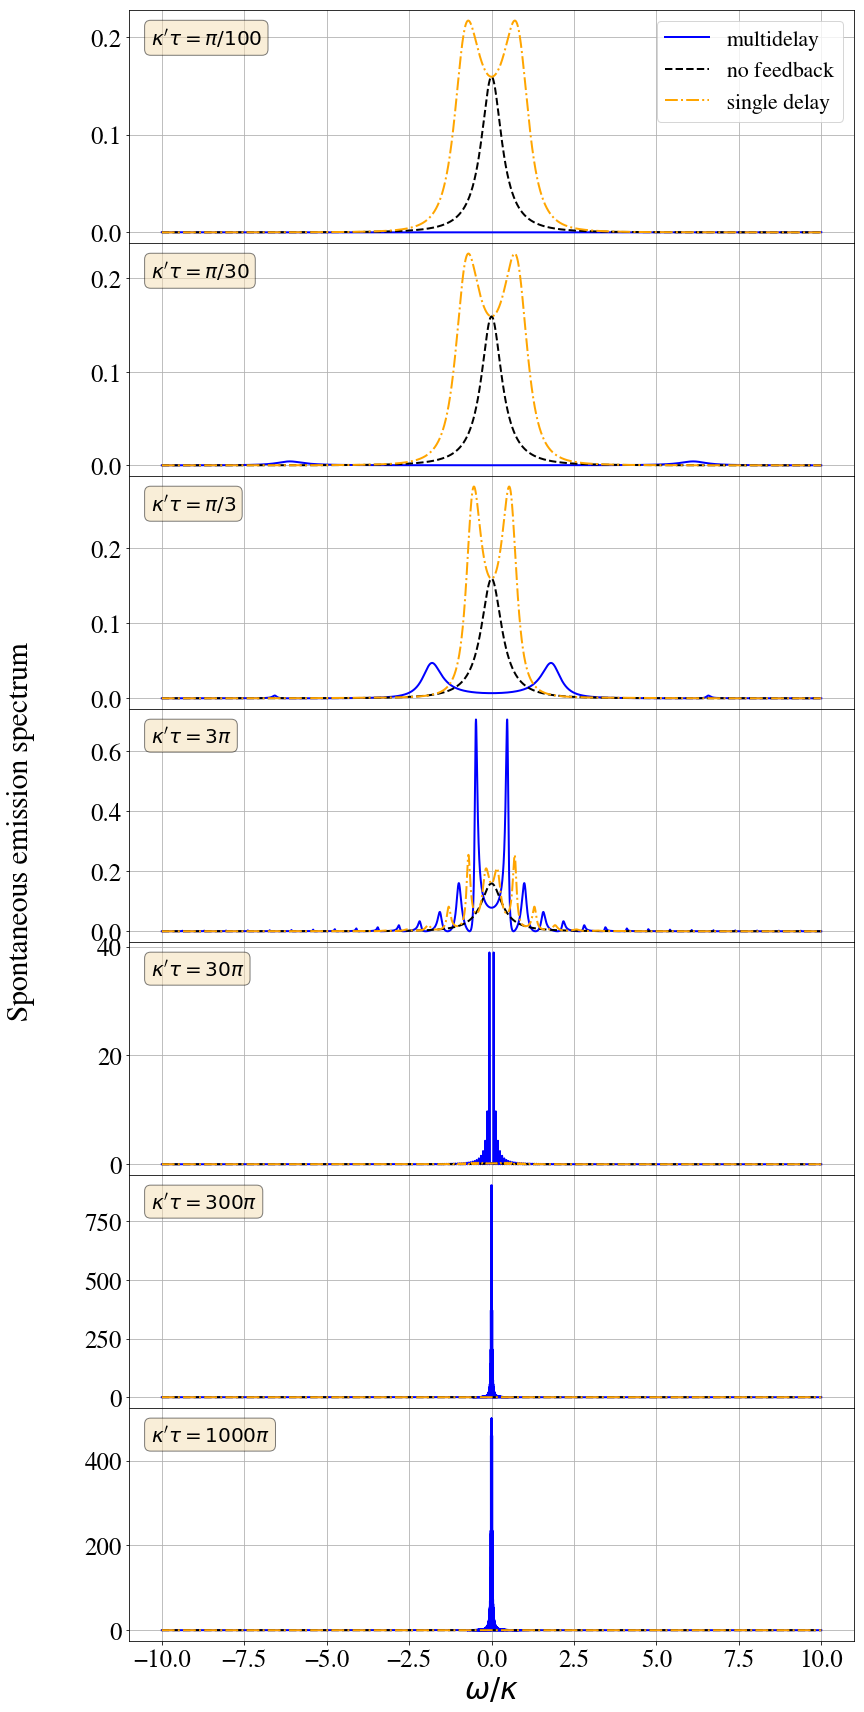
\includegraphics[width=0.56\textwidth]{spont_em_weak_highres.png}
%\vglue -.8 cm
%\label{fig:spontem_weak}
%\textit{\textbf{\caption{\linespread{1}\small{Time-evolution of the cavity field for different length of time-delay, when $\gamma=40\kappap=40\cdot 2\pi MHz$. The single-delay case is calculated from \cite{Kabuss2015}.}}}}
%\vglue -.1 cm
%\end{figure}
%\clearpage
%\begin{figure}[tb]
%\centering
%\vglue -.2 cm
%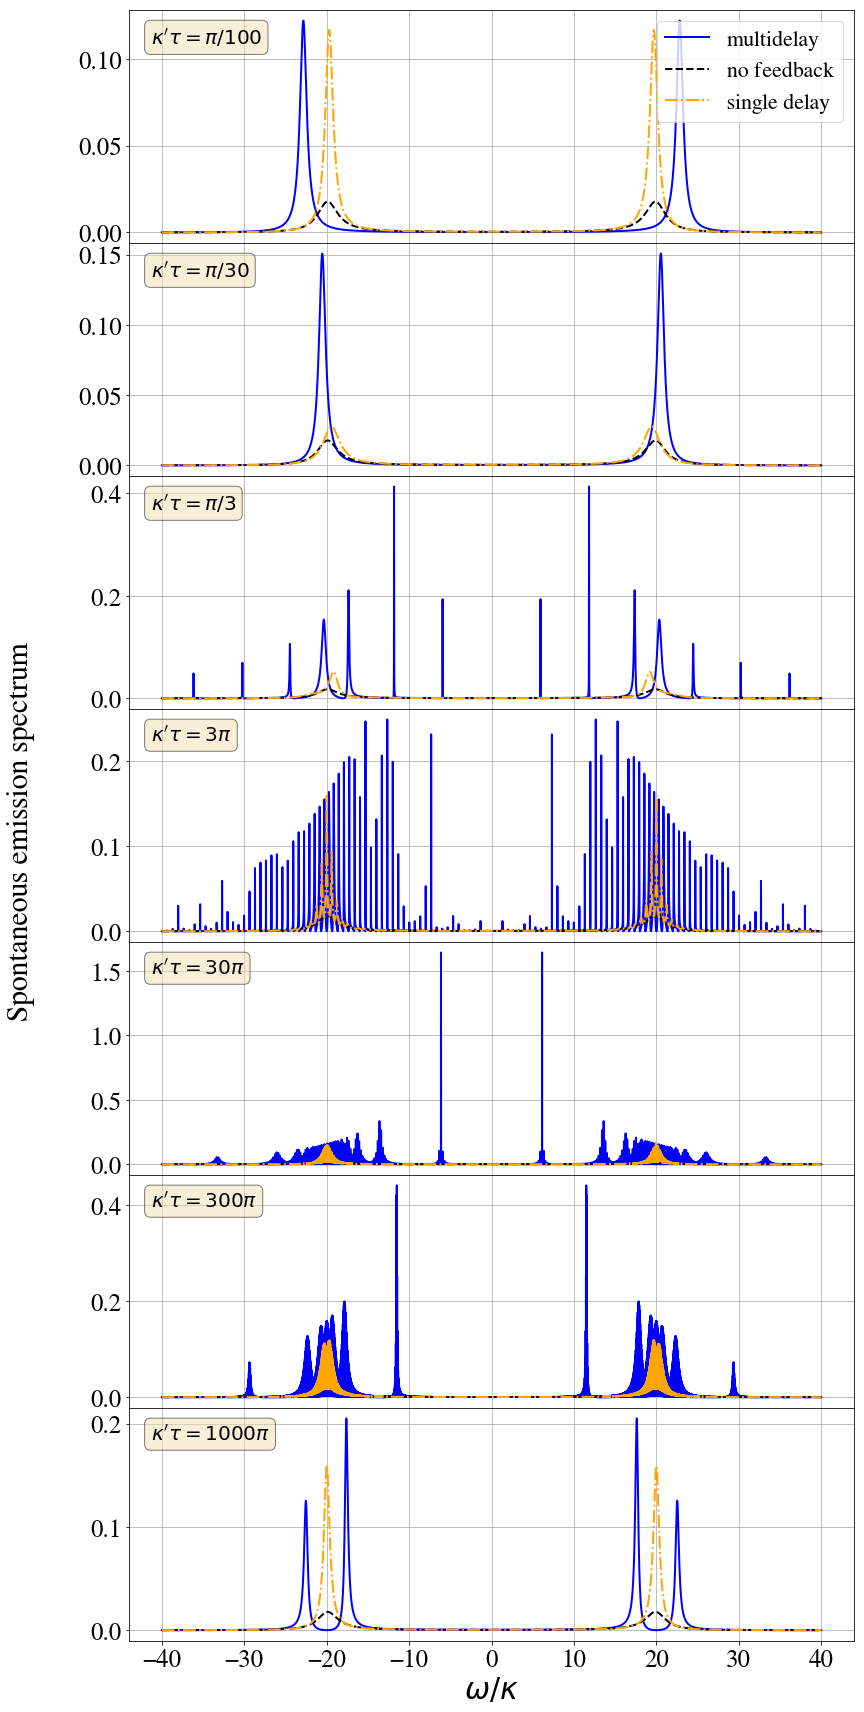
\includegraphics[width=0.56\textwidth]{spont_em_strong.png}
%\vglue -.8 cm
%\label{fig:strong_cavtls}
%\textit{\textbf{\caption{\linespread{1}\small{Time-evolution of the cavity field or different length of time-delay, when $\gamma=40\kappap=40\cdot 2\pi MHz$. The single-delay case is calculated from \cite{Kabuss2015}.}}}}
%\vglue -.1 cm
%\end{figure}
%\end{widetext}

\section{Conclusion}

\appendix
\section{Comparison between Dirac comb and wave number sum}
\note{Here we can put a plot to show how these two cases match each other.}

\section{Long-time solution in the weak coupling regime}
When $\gamma=\kappap$, the time-evolution of the system can be expressed by using the same tricks as in \cite{Kabuss2015}: \note{Recalculate this!}
\begin{align}
\label{eq:analytic}
c_g^{(\infty)}(t) &= i\sum_{m=0}^\infty\sum_{l=0}^m\sum_{p=0}^\infty(-4)^m\frac{m(p+m-1)!}{p!l!(m-l)!}\cdot\nn\\
&\hspace{.4cm}\cdot\frac{\lsz\kappa(t-p\tau)\rsz^{m+l+1}}{(m+l+1)!}e^{\kappa(t-p\tau)}\Theta(t-p\tau)
\end{align}

\note{Compare with single-delay case}

\bibstyle{apsrev4-1}
\bibliography{multidelay}

\end{document}
%
% ****** End of file apssamp.tex ******